\chapter{検出器量産と品質試験}
この章ではモジュールの組み立て工程と品質試験について説明する。

\section{組み立て工程}\label{sec:assembly}
モジュール組み立て機関は、初めにベアモジュールとフレキシブル基板を受け取る。
組み立て工程として以下が設定されている。
\begin{enumerate}
  \item フレキシブル基板・ベアモジュール貼り付け
  \begin{itemize}
    \item 受け取ったベアモジュールとフレキシブル基板を接着剤を用いて貼り付ける。
  \end{itemize}
  \item ワイヤー配線
  \begin{itemize}
    \item ワイヤー配線を行い、FEチップとフレキシブル基板を電気的に接続する。
  \end{itemize}
  \item ワイヤー保護
  \begin{itemize}
    \item ワイヤーが損傷があり断線が起きると、そのワイヤーに接続されているピクセルの読み出しができなくなる。これを防ぐため、モジュールに屋根型の構造を取り付け、ワイヤーを物理的に保護する。
  \end{itemize}
  \item パリレンコーティング
  \begin{itemize}
    \item モジュール読み出し部以外での電通や放電を防ぐため、パリレン高分子を用いてモジュールを保護する。
  \end{itemize}
  \item 温度サイクル試験
  \begin{itemize}
    \item ITk運転時の環境温度は$-45^\circ$Cから$40^\circ$Cまで変化しうる\cite{3-2}。この温度変化に耐えうるかを確認するため、温度サイクルを行う。
  \end{itemize}
  \item 低温耐久試験
  \begin{itemize}
    \item ITk運転時の典型的な環境温度は$-15〜0^\circ$C付近である。これに耐えうる性能を持つかを確認するために、低温下にモジュールを長時間設置する耐久試験を行う。
  \end{itemize}
\end{enumerate}

流れと各組み立て工程のイメージを図\ref{assembly_flow}に示す。
\begin{figure}[bpt]\centering
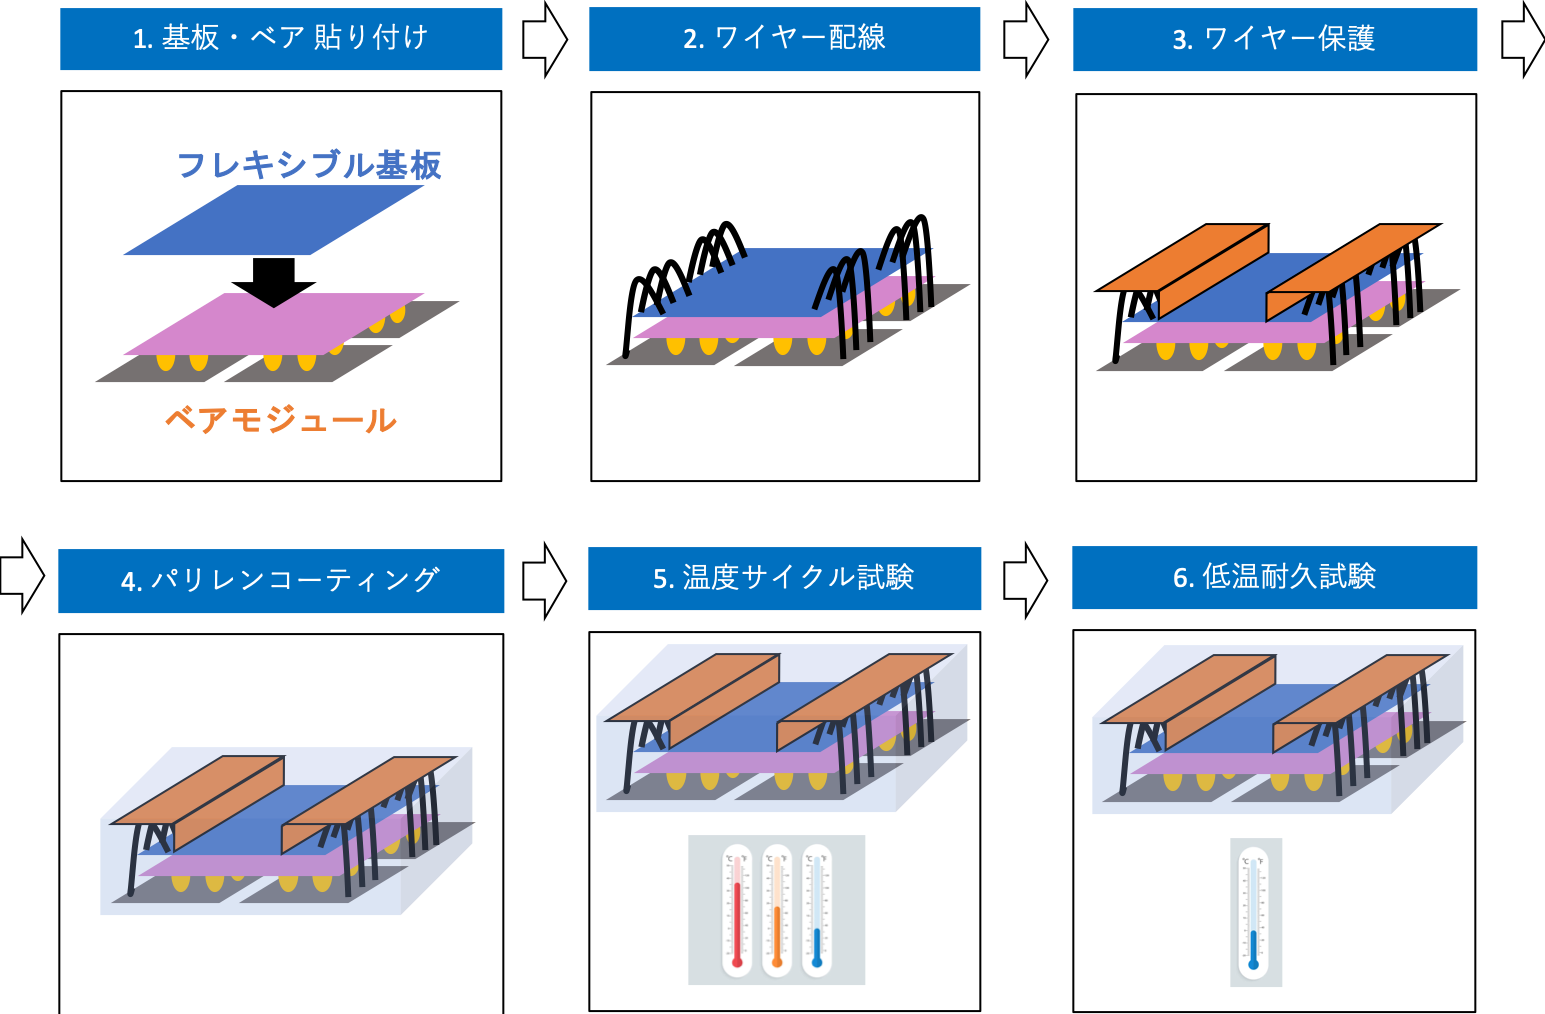
\includegraphics[width=12cm]{assembly_flow}
\caption[組み立て工程のイメージ図]{組み立て工程のイメージ図。モジュール組み立て機関はベアモジュール、フレキシブル基板を受け取り、それらの貼り付け、ワイヤー配線、ワイヤー保護、パリレンコーティング、温度サイクル試験、低温耐久試験の順に組み立てを行う。}
\label{assembly_flow}
\end{figure}

\section{品質試験}
各組み立て工程に対して、いくつかの品質試験を行う。行う品質試験の代表的なものを以下に示す。

\subsection{外観検査}
モジュールの外観写真を撮り、モジュールに以下のような欠陥がないかを確認する。
また外観検査の様子を図\ref{VI_overview}に示す。
\begin{itemize}
  \item 抵抗等取り付け部品の損傷.
  \item ワイヤーの接着位置確認.
  \item 基板上の回路やワイヤーの断線.
  \item 付着汚れ.
\end{itemize}

\begin{figure}[bpt]\centering
  \begin{minipage}{0.4\hsize}
    \begin{center}
    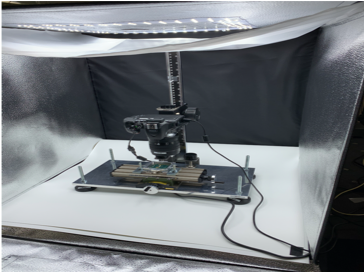
\includegraphics[width=60mm]{VI_setup}
    \end{center}
  \end{minipage}
  \begin{minipage}{0.4\hsize}
    \begin{center}
    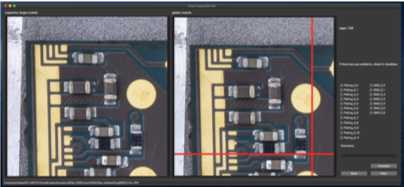
\includegraphics[width=65mm]{VI_analysis}
    \end{center}
  \end{minipage}
  \caption[外観検査の様子]{外観検査の様子。図は日本で実際に行われた外観検査における写真撮影の様子(左図)と撮影写真の確認画面(右図)である。左図のように、写真撮影は光量を制御するため暗箱の中で行っている。またモジュールに損傷や断線がないかを確認するために、右図のように撮影した写真と良好なモジュールの写真を見比べ、電子部品の損傷、回路の断線などの何らかの所見があった場合には記録をする。}
  \label{VI_overview}
\end{figure}

\subsection{質量測定}
モジュールの質量を測定する試験である。

\subsection{平坦性測定}
モジュール上の位置座標を何点か測定し、モジュールの平坦度、厚さ、歪み具合等を測定する。
測定の様子と解析の例を図\ref{Metrology_overview}に示す。

\begin{figure}[bpt]\centering
  \begin{minipage}{0.4\hsize}
    \begin{center}
    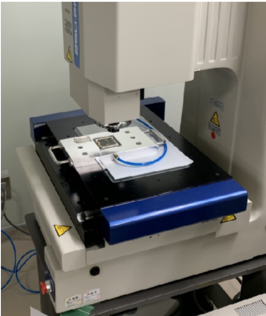
\includegraphics[width=60mm]{Metrology_setup}
    \end{center}
  \end{minipage}
  \begin{minipage}{0.4\hsize}
    \begin{center}
    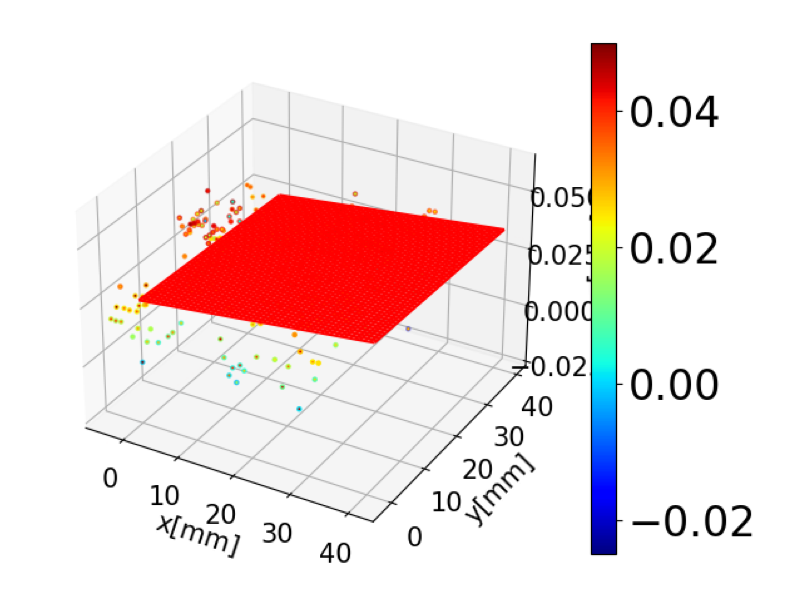
\includegraphics[width=65mm]{Metrology_analysis}
    \end{center}
  \end{minipage}
  \caption[平坦性測定の様子。]{平坦性測定の様子。図は日本で実際に行われた平坦性測定における測定の様子(左図)と解析結果(右図)である。専用の装置を用いてモジュールの位置座標を何点か測定する。得られた測定点は右図のように図示し、平面でフィッティングを行う。フィット平面からのズレの分布や、モジュールの厚みを計算する。}
  \label{Metrology_overview}
\end{figure}

\clearpage
\subsection{センサー電流-電圧特性確認}
モジュールのシリコンセンサーに逆バイアス電圧をかけ、電流-電圧特性をみる。
印加電圧を段階的に変化させて測定点をとり、電流と電圧の関係を確認する。
この試験の結果の例を図\ref{sensor_IV_result}に示す。
逆方向電圧では電流はほとんど流れないが、降伏電圧に達すると急激に増大する。
これはpn接合の特性\cite{2-1}であり、正常であればこの振る舞いを確認することができる。

\begin{figure}[bpt]\centering
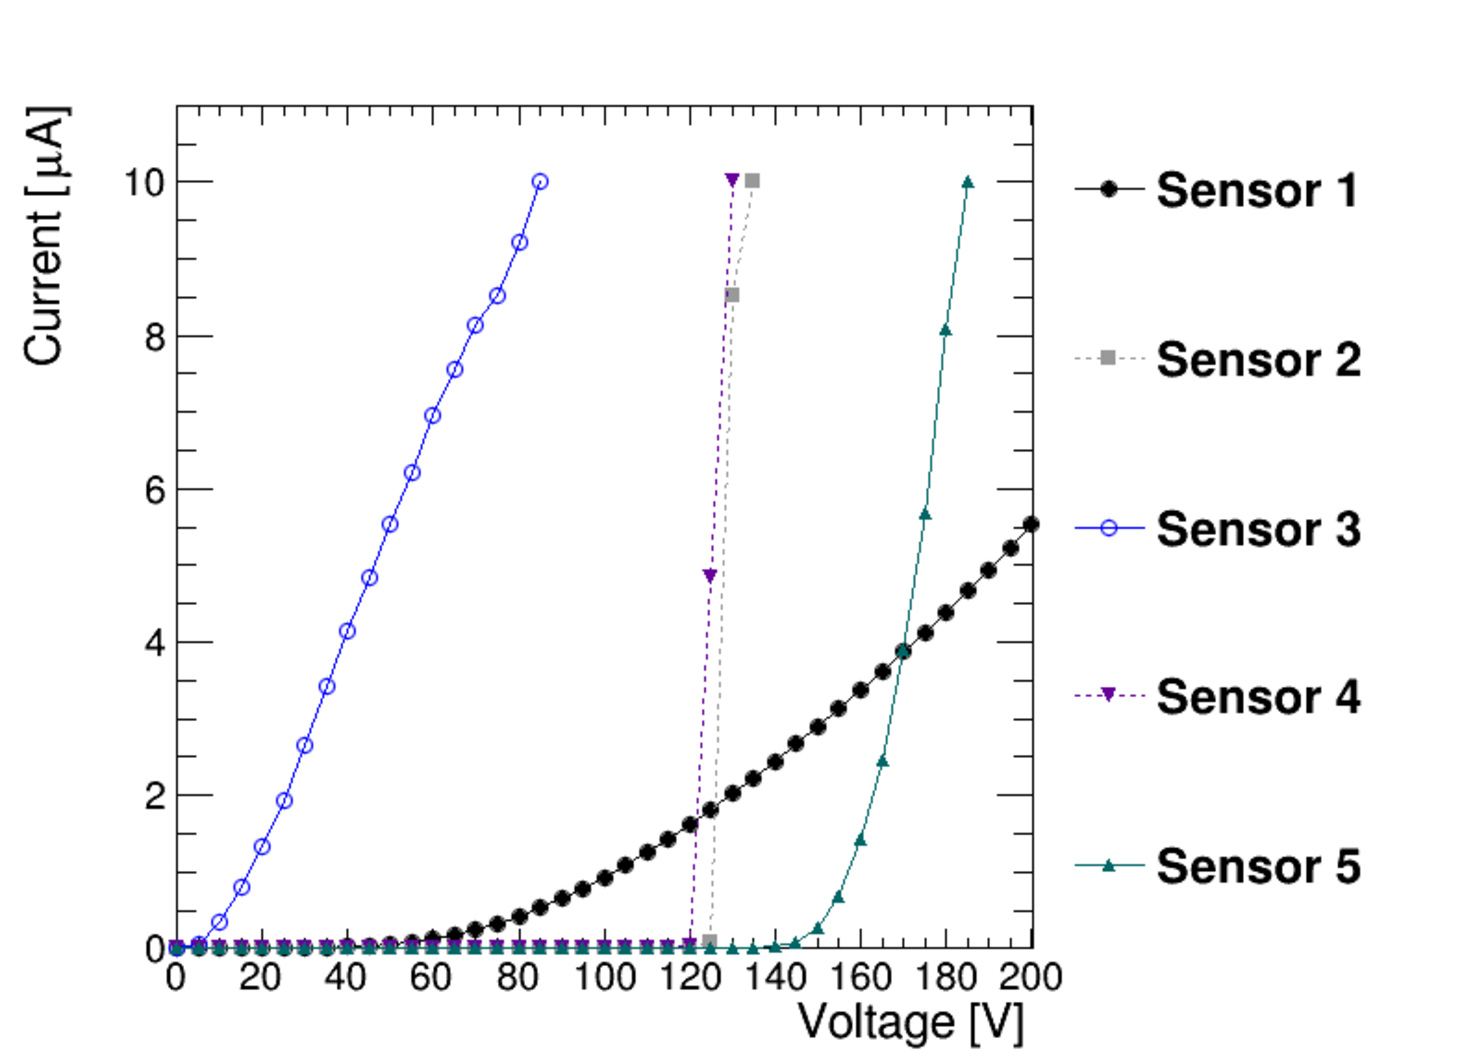
\includegraphics[width=7cm]{sensor_IV_result}
\caption[センサー電流-電圧特性結果の例]{センサー電流-電圧特性結果の例\cite{3-4}。横軸にセンサーに対する印加電圧[V]、縦軸に電流[$\mu$A]を示す。逆バイアス電圧を印加しているため、電流が0Vから60V付近までは電流がほとんど流れていないが、70V付近から電流が急激に増加していることが分かる。}
\label{sensor_IV_result}
\end{figure}

\subsection{FEチップ電流-電圧特性確認}
FEチップに対して電圧をかけ、電流-電圧特性をみる。
センサーに対してと同様に、印加電圧を段階的に変化させて測定点をとり、電流と電圧の関係を確認する。
抵抗として振る舞うため、電流、電圧間の関係は図\ref{SLDO_VI_result}のように線形性を持つ。

\begin{figure}[bpt]\centering
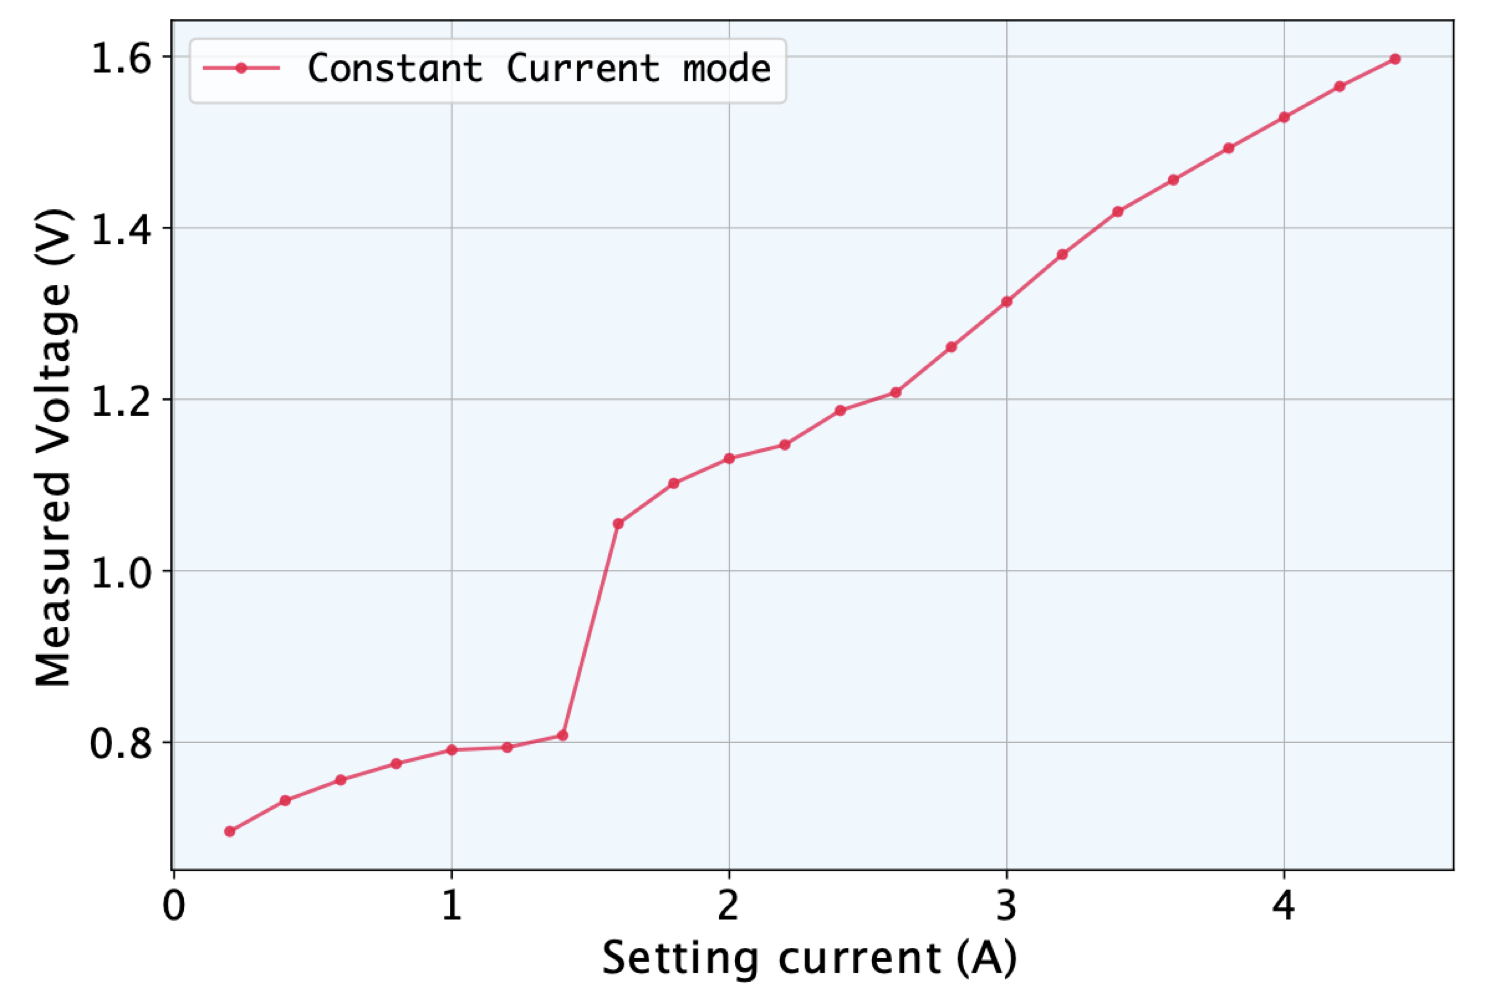
\includegraphics[width=7cm]{SLDO_VI_result}
\caption[FEチップ電流-電圧特性試験結果の例。]{FEチップ電流-電圧特性試験結果の例\cite{3-4}。横軸にFEチップに対する設定電流、縦軸は測定した実際にFEチップにかかる電圧値を示している。1.5V付近に急激に電圧が増大しており、この段階でFEチップが機能するようになる。それ以降は線形になっているのが分かる。}
\label{SLDO_VI_result}
\end{figure}

\clearpage
\subsection{読み出し試験}
読み出し試験では、読み出し回路が正常に機能するのかを確認する。
読み出し試験の様子を図\ref{readout_overview}に示す。モジュールに読み出しケーブルを配線し、PCと通信を行い、データを取得する。
また試験において温度、FEチップやセンサーに与える電圧、電流といった検出器の操作、環境関わる情報取得を同時に行い、異常がないかを確認する。これらの情報は「\textbf{Detector Control System, DCS}」と呼ぶ。

\begin{figure}[bpt]\centering
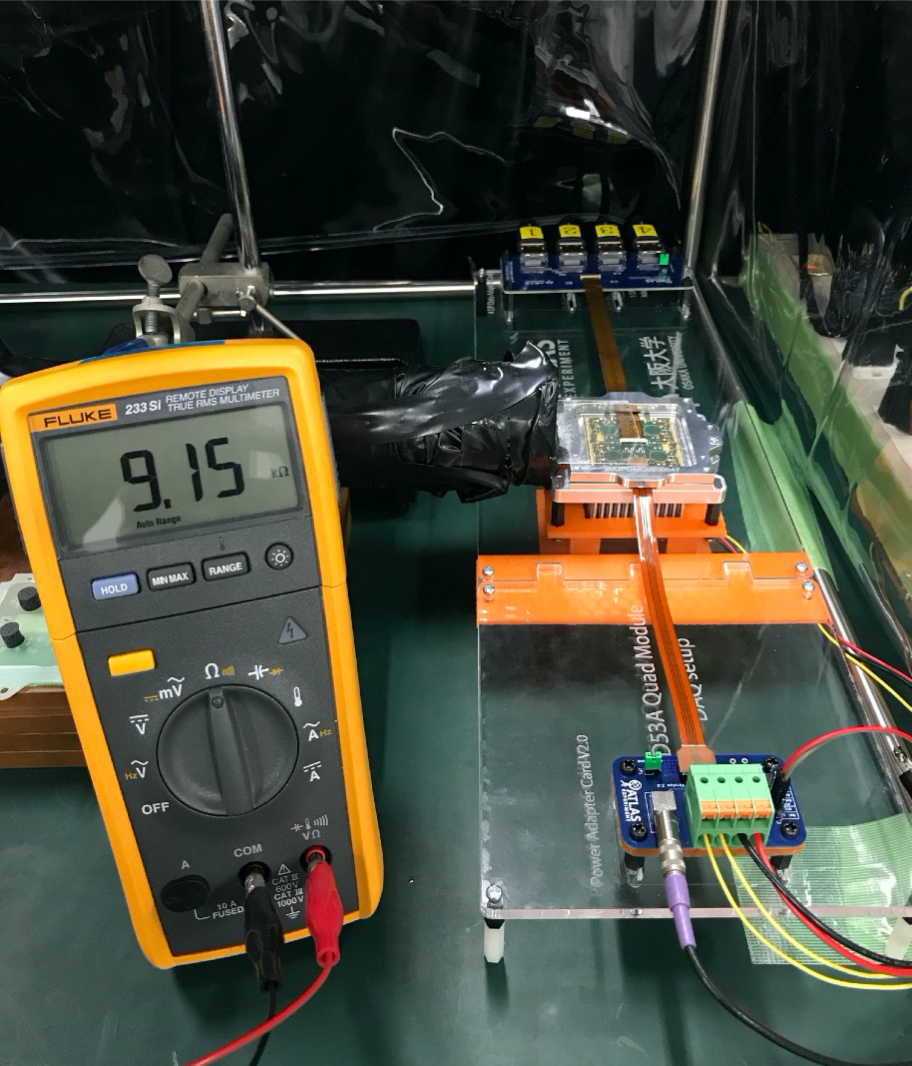
\includegraphics[width=7cm]{readout_overview}
\caption[読み出し試験の様子]{読み出し試験の様子\cite{3-4}。図は日本で実際に行われた読み出し試験の様子である。図の右側に見えるように、モジュールにケーブルを配線し、PCとの通信を行うことでデータ取得をする。また図の左側では抵抗値を測定している。これはモジュールに付属しているサーミスタの抵抗値を確認することで、温度情報を取得するためのものである。}
\label{readout_overview}
\end{figure}

\subsubsection{汎用読み出しシステムYARR}
\textbf{YARR(Yet Another Rapid Readout)}システム\cite{3-3}は、ピクセルモジュール用に開発された、PCI Express(PCIe)接続を用いた読み出しシステムである。
ファームウェア、ソフトウェアから構成される。YARRではファームウェア上で行う処理はデータ通信やトリガー処理等の最低限に抑え、その他多くの処理をソフトウェアで担うという特徴がある。

\subsubsection{読み出し試験に使用するファイルと変数}
YARRで扱う全てのファイルは\textbf{JSON(JavaScript Object Notation)}と呼ばれる形式で記述される。

YARRを用いた読み出し試験では以下の設定ファイルが要求される。
\begin{itemize}
  \item 試験設定ファイル
  \begin{itemize}
    \item 読み出し試験の初期設定や解析手法を記述する。
  \end{itemize}
  \item ハードウェア設置ファイル
  \begin{itemize}
    \item 試験に用いるハードウェアの指定や設定を記述する。
  \end{itemize}
  \item 接続設定ファイル
  \begin{itemize}
    \item 読み出しを行うFEチップの種類やチャンネルを記述する。
  \end{itemize}  
  \item FEチップ設定ファイル.
  \begin{itemize}
    \item 各FEチップ毎に出力され、全ピクセルに共通な試験の設定値、各ピクセル固有の設定値を記述する。
  \end{itemize}  
\end{itemize}

また試験1項目ごとに以下のファイルが、1つのディレクトリに生成される。
\begin{itemize}
  \item 試験結果ファイル.
  \begin{itemize}
    \item 各ピクセルのOccupancy等、読み出し試験の結果値を記述する。
  \end{itemize}
  \item 試験設定ファイル
  \item FEチップ設定ファイル.
  \begin{itemize}
    \item 試験の中で変更が加えられるため、各FEチップにつき試験前後の2つのファイルが出力される。
  \end{itemize}
  \item 試験ログ
  \begin{itemize}
    \item 試験情報を記録する。
  \end{itemize}
\end{itemize}

後述するローカルデータベースシステムにおいてはさらに以下の設定ファイルを用いる。
\begin{itemize}
  \item データベース設定ファイル.
  \item 試験者設定ファイル. 
  \item 試験場所設定ファイル.
\end{itemize}

読み出し試験項目において以下の$Occupancy$という量が定義される。
試験用電荷の入射数や発行トリガーの数等、発行した信号数を$n_i$回、取得信号数を$n_0$としたとき、
\bbb
\label{occupancy}
Occupancy = \frac{n_0}{n_i} \times 100~[\%]
\eee
と定義する。


また読み出し試験では各FEチップに対して「\textbf{レジスタ}」と呼ばれる設定値が存在し、FEチップ上の全ピクセルに対して共通なものを「\textbf{グローバルレジスタ}」、各ピクセル固有のものを「\textbf{ピクセルレジスタ}」と呼ぶ。

\clearpage
\subsubsection{読み出し試験項目}
以下に読み出し試験項目の一覧を示す。
\begin{description}
  \item[レジスタの読み書き]\mbox{}\\
グローバル及びピクセルレジスタの読み書きが正常にできるのかを確認する試験.
  \item[デジタル回路読み出し]\mbox{} \\
各ピクセルのデジタル回路部に試験用電荷を入射し、信号の応答数を確認する試験. デジタル回路部の性能確認に用いる.
  \item[アナログ回路読み出し]\mbox{}\\
各ピクセルのアナログ回路部に試験用電荷を入射し、信号の応答数を確認する試験. アナログ回路部の性能確認に用いる.
  \item[Threshold測定]\mbox{}\\
各ピクセルのThreshold値を測定する試験.
  \item[Thresholdグローバルレジスタ調整]\mbox{}\\
全ピクセルに共通なレジスタの変更、基準となるThresholdに近づけるための調整.
  \item[Thresholdピクセルレジスタ調整、再調整、精密調整]\mbox{}\\
各ピクセル固有のレジスタの変更、基準となるThresholdに近づけるための調整.
  \item[ToTグローバルレジスタ調整]\mbox{}\\
全ピクセルに共通なレジスタの変更、基準となるToTに近づけるための調整.
  \item[ノイズ占有率測定]\mbox{}\\
各ピクセルのノイズの頻度を確認する試験.
  \item[スタックピクセル測定]\mbox{}\\
入力電荷の有無にかかわらず、常に信号を出力するピクセルを確認する試験.
  \item[クロストーク測定]\mbox{}\\
各ピクセルのクロストークの有無を確認する試験.
  \item[バンプ接続確認測定]\mbox{}\\
各ピクセルのバンプ接合が正常かを確認する試験.
  \item[外部トリガーを用いた測定]\mbox{}\\
外部トリガーを用いて信号の取得を行う試験.放射線源を用いた測定に使用.
\end{description}

主な試験項目の詳細について以下で説明する。

\subsubsection{デジタル回路読み出し}
各ピクセルのデジタル回路部に試験用電荷を入射し、信号を取得する。
$Occupancy$(式\ref{occupancy})は、入射電荷数$n_i$と取得信号数$n_0$で定義される。

デジタル回路読み出しにおける$Occupancy$の二次元分布の例を図\ref{dig_occ}に示す。
\begin{figure}[bpt]\centering
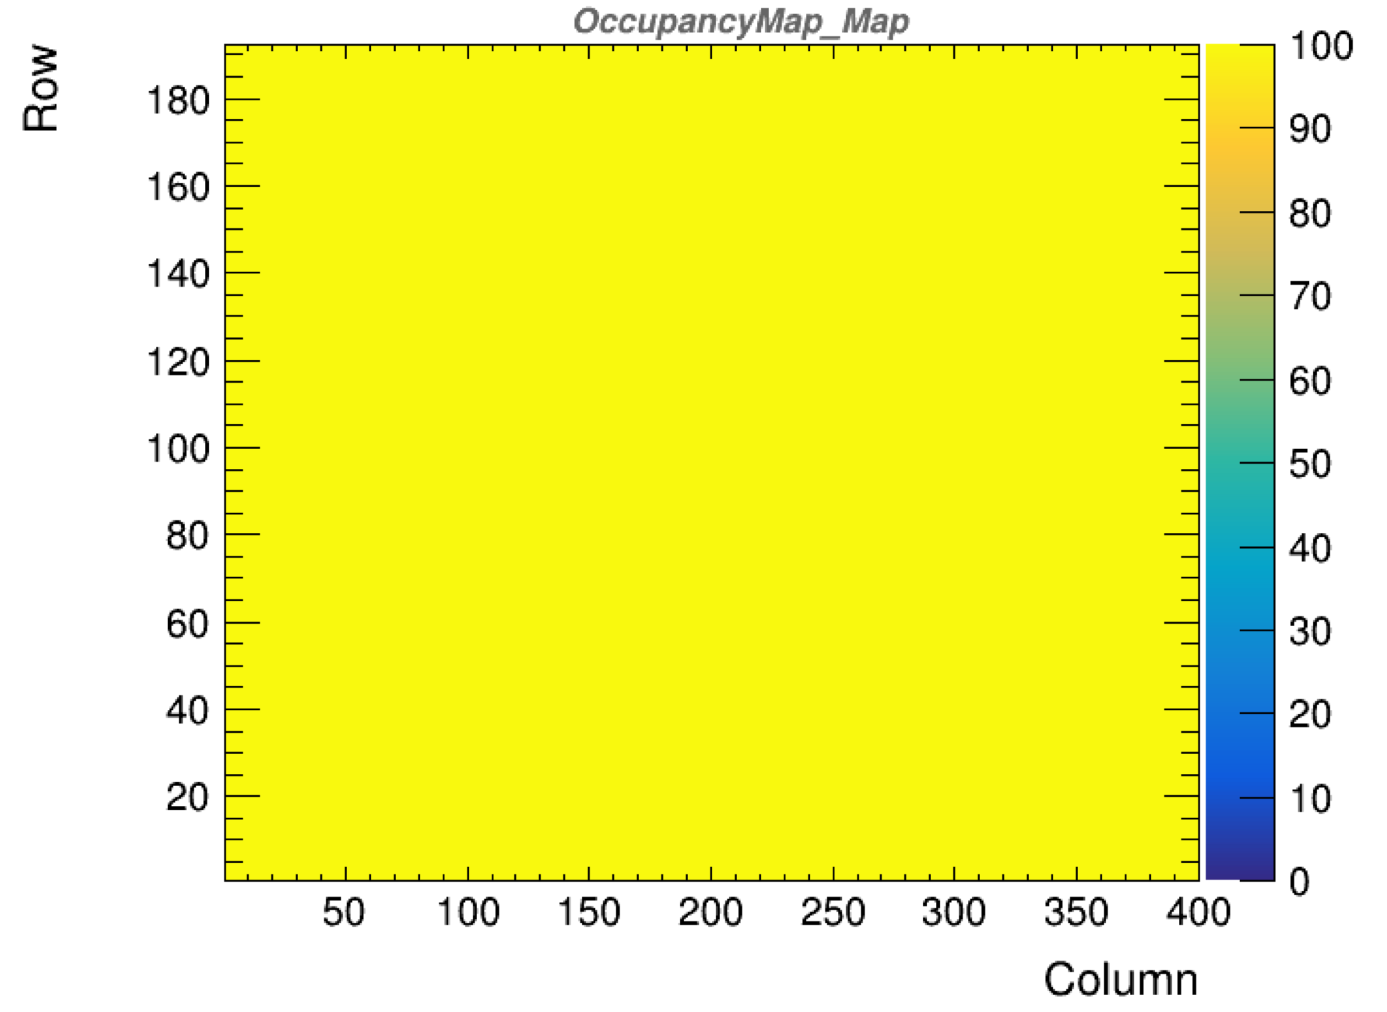
\includegraphics[width=8cm]{dig_occ}
\caption[デジタル回路読み出しにおける$Occupancy$分布の例。]{デジタル回路読み出しにおける$Occupancy$分布の例。図はRD53Aを用いたデジタル回路読み出しの結果であり、横軸、縦軸はそれぞれピクセルの列(400)、行(192)に対応する。z軸は各ピクセルにおける$Occupancy$の値を示している。正常なピクセルは100付近になることが期待され、図では全てのピクセルで100であるとが分かる。}
\label{dig_occ}
\end{figure}

この試験の結果として出力されるファイルを以下に示す。
\begin{description}
  \item [OccupancyMap] 各ピクセルの$Occupancy$を記す.
  \item [Enmask] $Occupancy=100$のピクセルを1、それ以外を0とした値を記す.
  \item [L1Dist] 信号取得タイミングの分布を記す.
\end{description}

\subsubsection{アナログ回路読み出し}
各ピクセルのアナログ回路部に試験用電荷を入射し、信号を取得する。
デジタル回路読み出しと同様、$Occupancy$(式\ref{occupancy})は、入射電荷数$n_i$と取得信号数$n_0$で定義される。
試験結果として出力されるファイルはデジタル回路読み出しと同じ形式である。

\subsubsection{Threshold測定}
各ピクセルのアナログ回路部に試験用電荷を入射し、入射電荷数$n_i$と取得信号数$n_0$より$Occupancy$を測定する。
これを入射電荷量を増加させて繰り返し行う。
あるピクセルにおけるこの処理結果の例を図\ref{threshold_scurve}に示す。
\begin{figure}[bpt]\centering
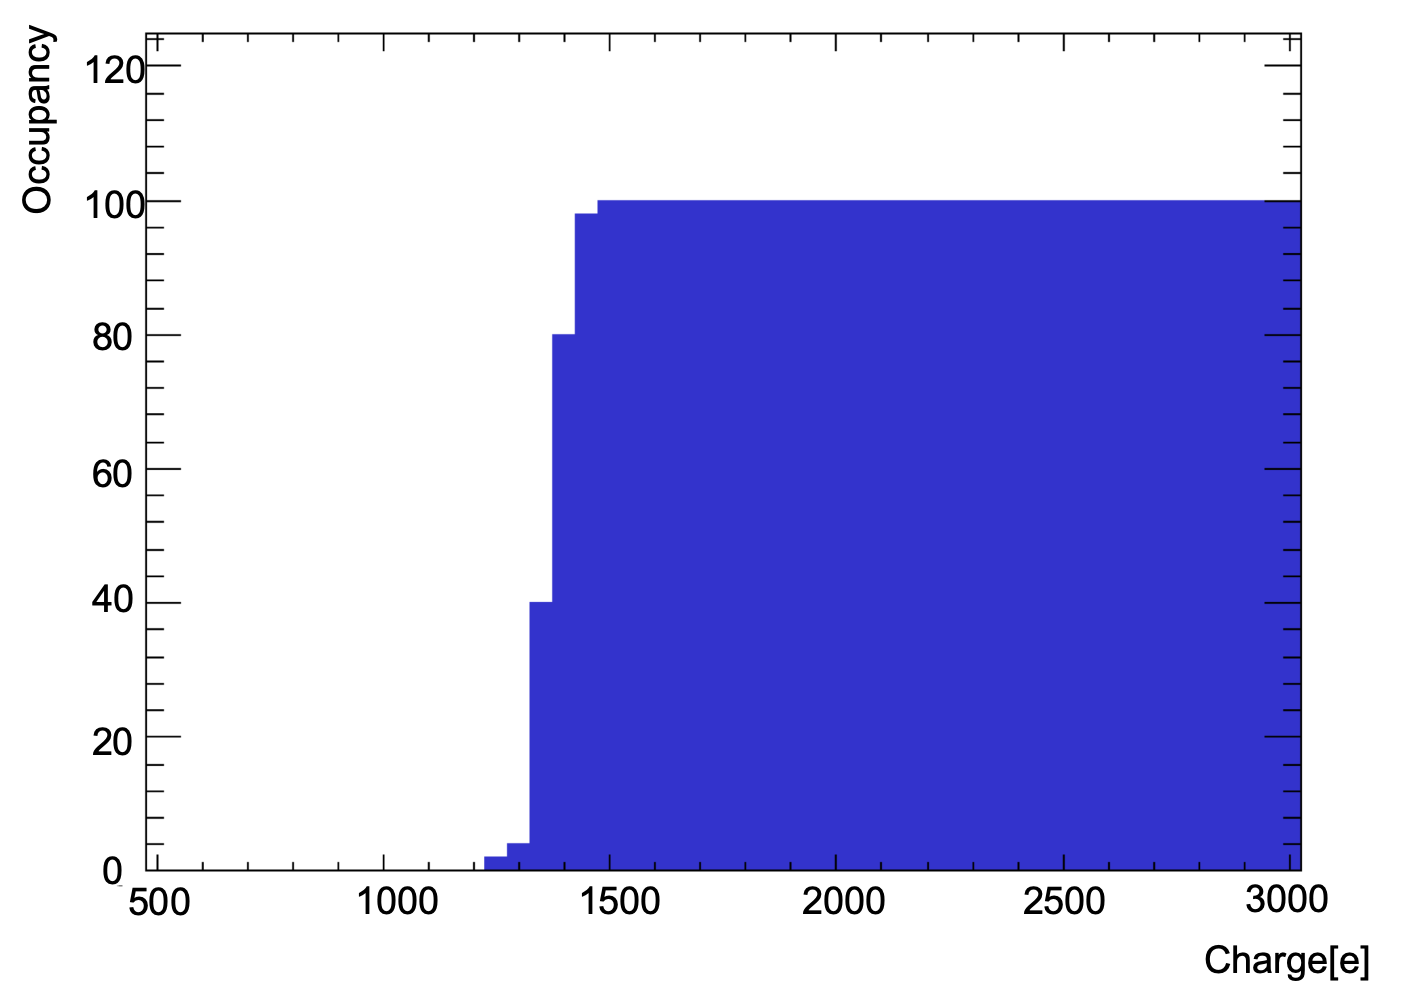
\includegraphics[width=8cm]{threshold_scurve}
\caption[入射電荷量と$Occupancy$の関係]{入射電荷量と$Occupancy$の関係。横軸はピクセルに対する入射電荷量[e]、縦軸は$Occupancy$を示す。入射電荷量の単位eは、電荷量Cを素電化$1.6\times 10^{-19}$で割ったものである。Threshold測定の際にはこのように入射電荷量を増加させながら$Occupancy$の値を測定する。測定結果を後述する式(\ref{scurve_function})フィットし、 Thresholdとノイズの値を得る。}
\label{threshold_scurve}
\end{figure}

この分布を以下の式でフィッティングする。フィッテングの形に由来し、これを「Sカーブフィッティング」と呼ぶ。
\bbb
\label{scurve_function}
f(x) &=& 0.5 \times \left[ 2-{\rm erfc}\left( \left\{ \frac{x-Q_{\rm th}}{\sigma_{\rm n} \times \sqrt{2}}  \right\} \right) \right] \times p\\
{\rm erfc}(x) &=& 1 - {\rm erf}(x)
%g(x) = \frac{2}{\sqrt{\pi}} \int_x^\infty {\rm exp}(-t^2) {\rm d}t
\eee
ここで${\rm erf}(x)$はガウスの誤差関数である\cite{3-5}。

得られた$Q_{\rm th}$、$\sigma_{\rm n}$がそれぞれピクセルのThreshold値、ノイズに相当する。
あるFEチップにおける$Q_{\rm th}$、$\sigma_{\rm n}$の分布の例を図\ref{threshold_mean_sigma}に示す。
この分布をガウス関数でフィットすることで、全ピクセルに対するThreshold、ノイズの平均値$Q_{\rm th,mean}、\sigma_{\rm n,mean}$、幅$Q_{\rm th,sigma}、\sigma_{\rm n,sigma}$が得られる。

\begin{figure}[bpt]\centering
  \begin{minipage}{0.45\hsize}
    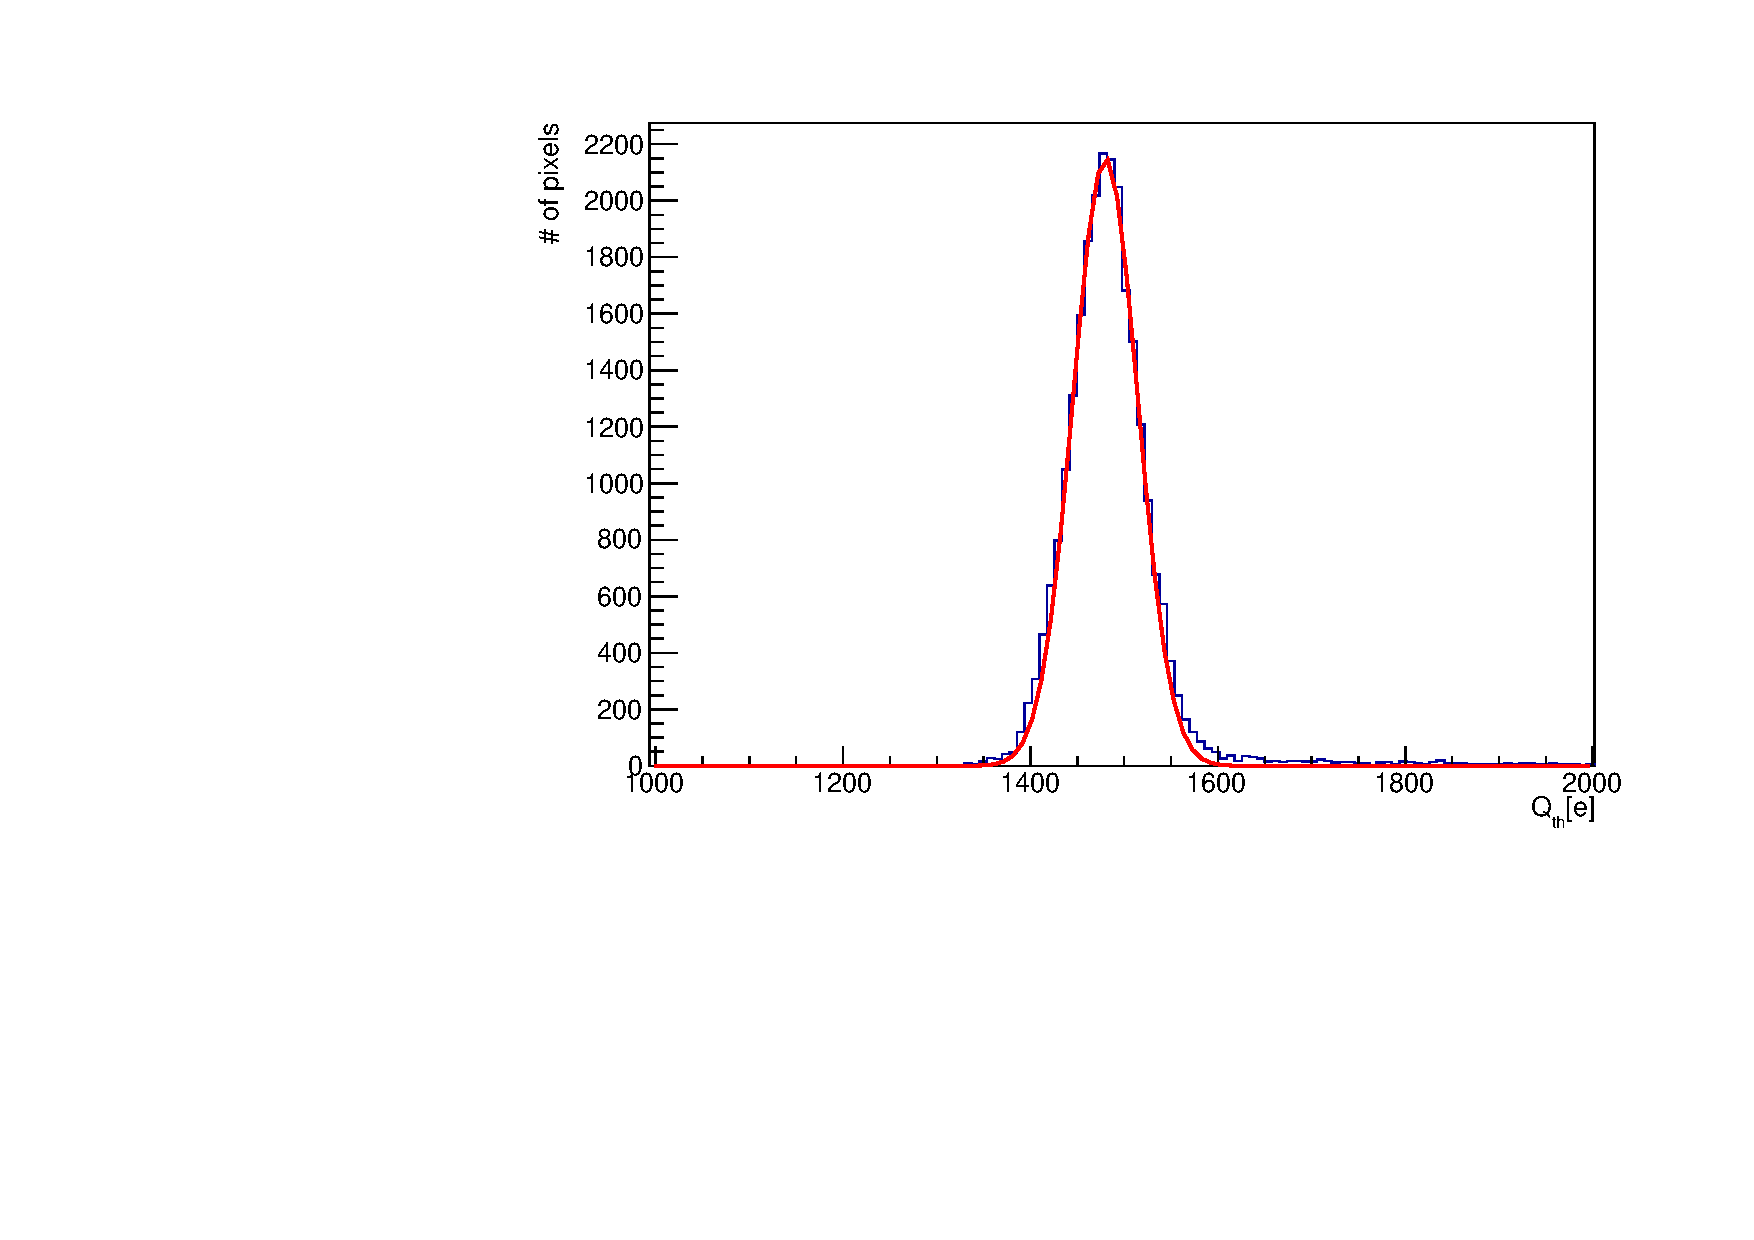
\includegraphics[width=50mm,angle=270]{Threshold_mean_dist}
  \end{minipage}
  \begin{minipage}{0.45\hsize}
    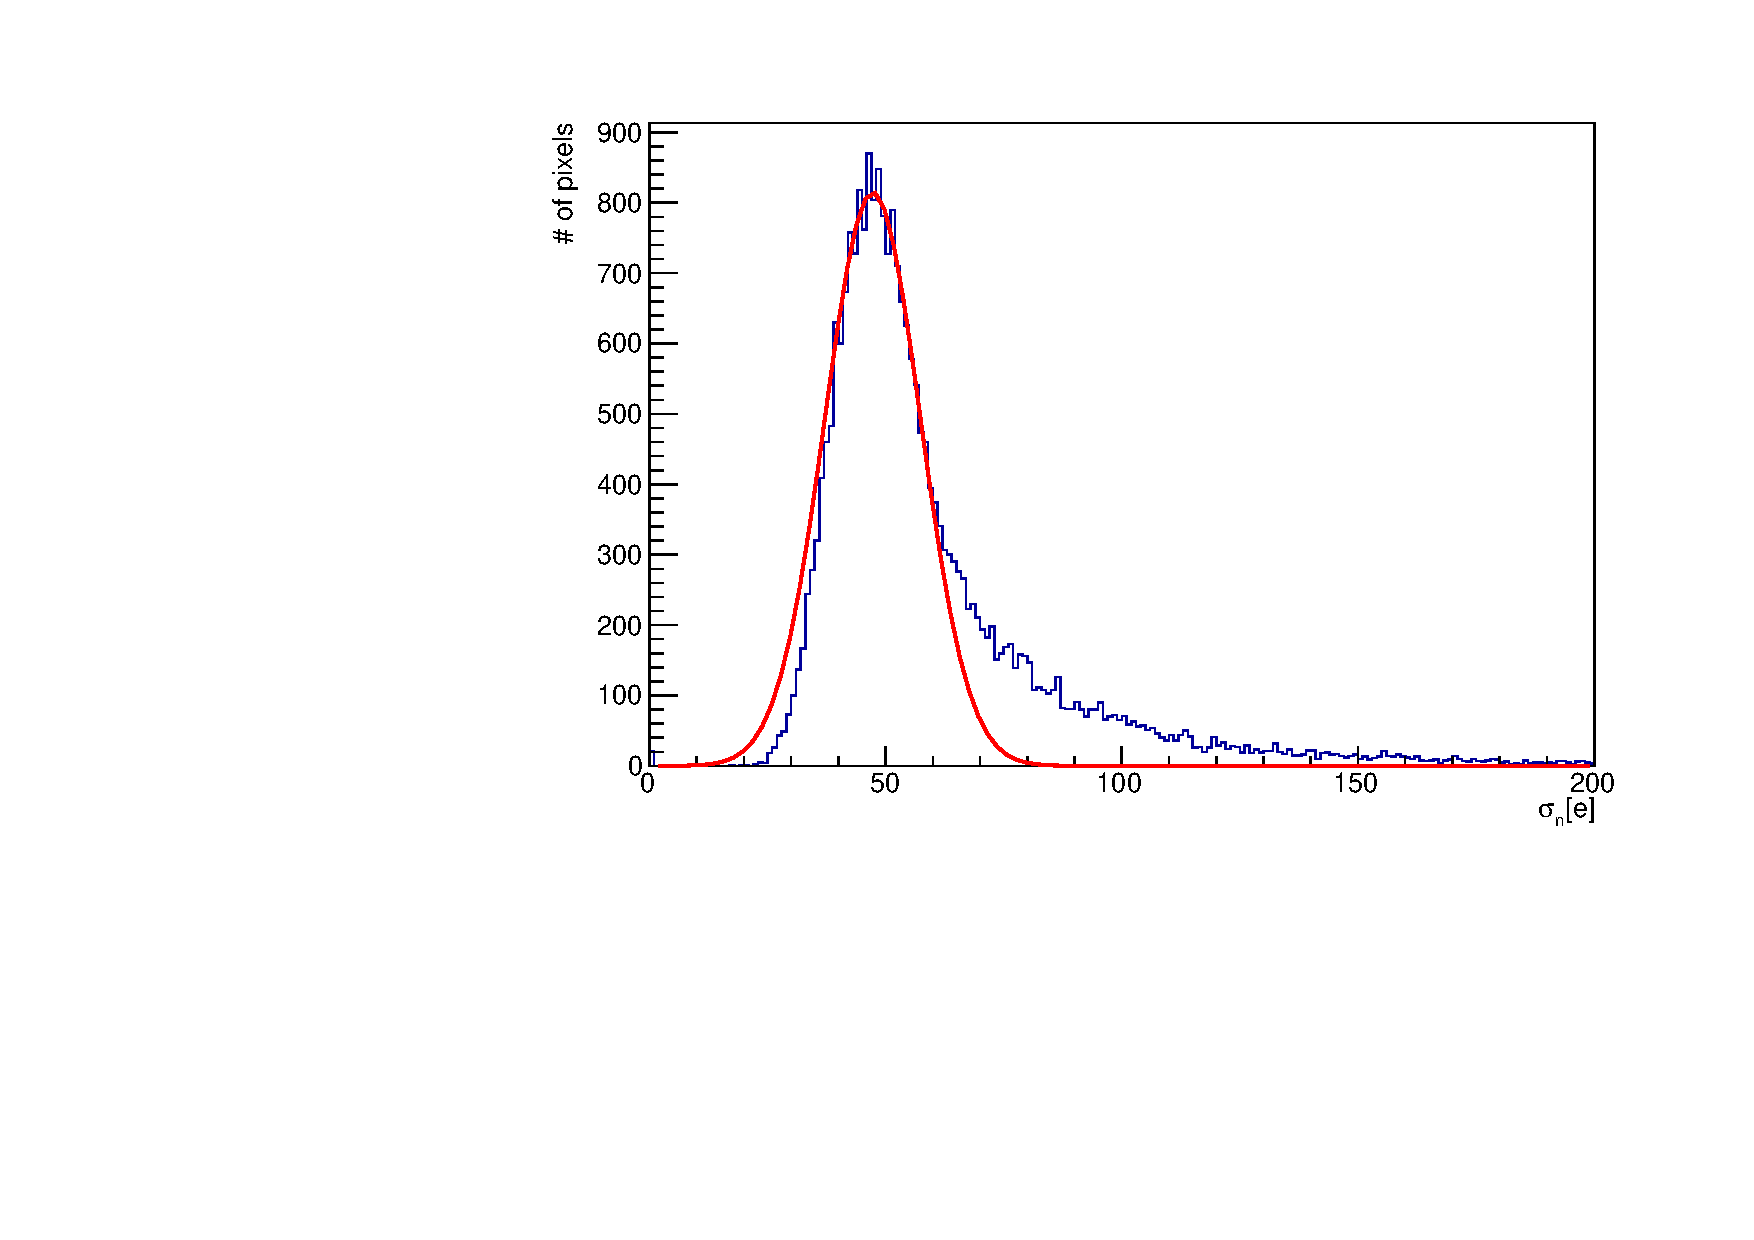
\includegraphics[width=50mm,angle=270]{Threshold_noise_dist}
  \end{minipage}
  \caption[Threshold値($Q_{\rm th}$)とノイズ($\sigma_{\rm n}$)の分布。]{Threshold値($Q_{\rm th}$)とノイズ($\sigma_{\rm n}$)の分布。図はあるFEチップ上のピクセルにおけるThreshold値($Q_{\rm th}$, 左図)とノイズ($\sigma_{\rm n}$,右図)の分布を示している。また赤線はガウス関数によるフィット関数を示しており、これにより平均値と幅を取得する。}
  \label{threshold_mean_sigma}
\end{figure}

この試験において、出力される結果ファイルを以下に示す。
\begin{description}
  \item [ThresholdMap] 各ピクセルの$Q_{\rm th}$を記す.
  \item [ThresholdDist] $Q_{\rm th}$の分布を記す.
  \item [NoiseMap] 各ピクセルの$\sigma_{\rm n}$を記す.
  \item [NoiseDist] $\sigma_{\rm n}$の分布を記す. 
  \item [Chi2Map] 各ピクセルのSカーブフィッティングにおける$\chi^2$の値を記す.
  \item [Chi2Dist] $\chi^2$の分布を記す.
  \item [sCurve] あるピクセルの入射電荷量と$Occupancy$の関係を記す. いくつかのピクセルについて出力する.
  \item [sCurveMap] 全てのピクセルのSCurveを重ね合わせた値を記す.
\end{description}

\subsubsection{ToT測定}
各ピクセルのアナログ回路部に試験用電荷を入射し、ToTを測定する。
複数回行い、平均値と幅を求める。
出力される結果ファイルを以下に示す。
\begin{description}
  \item [MeanToTMap] 各ピクセルのToTの平均値を記す.
  \item [MeanToTDist] ToT平均値の分布を記す. 
  \item [SigmaToTMap] 各ピクセルのToTの分散を記す.
  \item [SigmaToTDist] ToT分散の分布を記す.
\end{description}

\subsubsection{ノイズ占有率測定}
試験用電荷を入射せずに、$t$[sec]の時間トリガーをかけ、取得信号数$n_i$を測定する。
$Occupancy$(式\ref{occupancy})は、発行したトリガー数$n_i$と取得信号数$n_0$で定義される。

また$NoiseOccupancy$を以下で定義する。
$NoiseOccupancy$の分布の例を図\ref{noise_occ}に示す。
\bbb
NoiseOccupancy = \frac{n_i}{t} \times (25 \times 10^{-9})
\eee
$25 \times 10^{-9}[{\rm sec}]=25[{\rm nsec}]$は1~b.c.である。

\begin{figure}[bpt]\centering
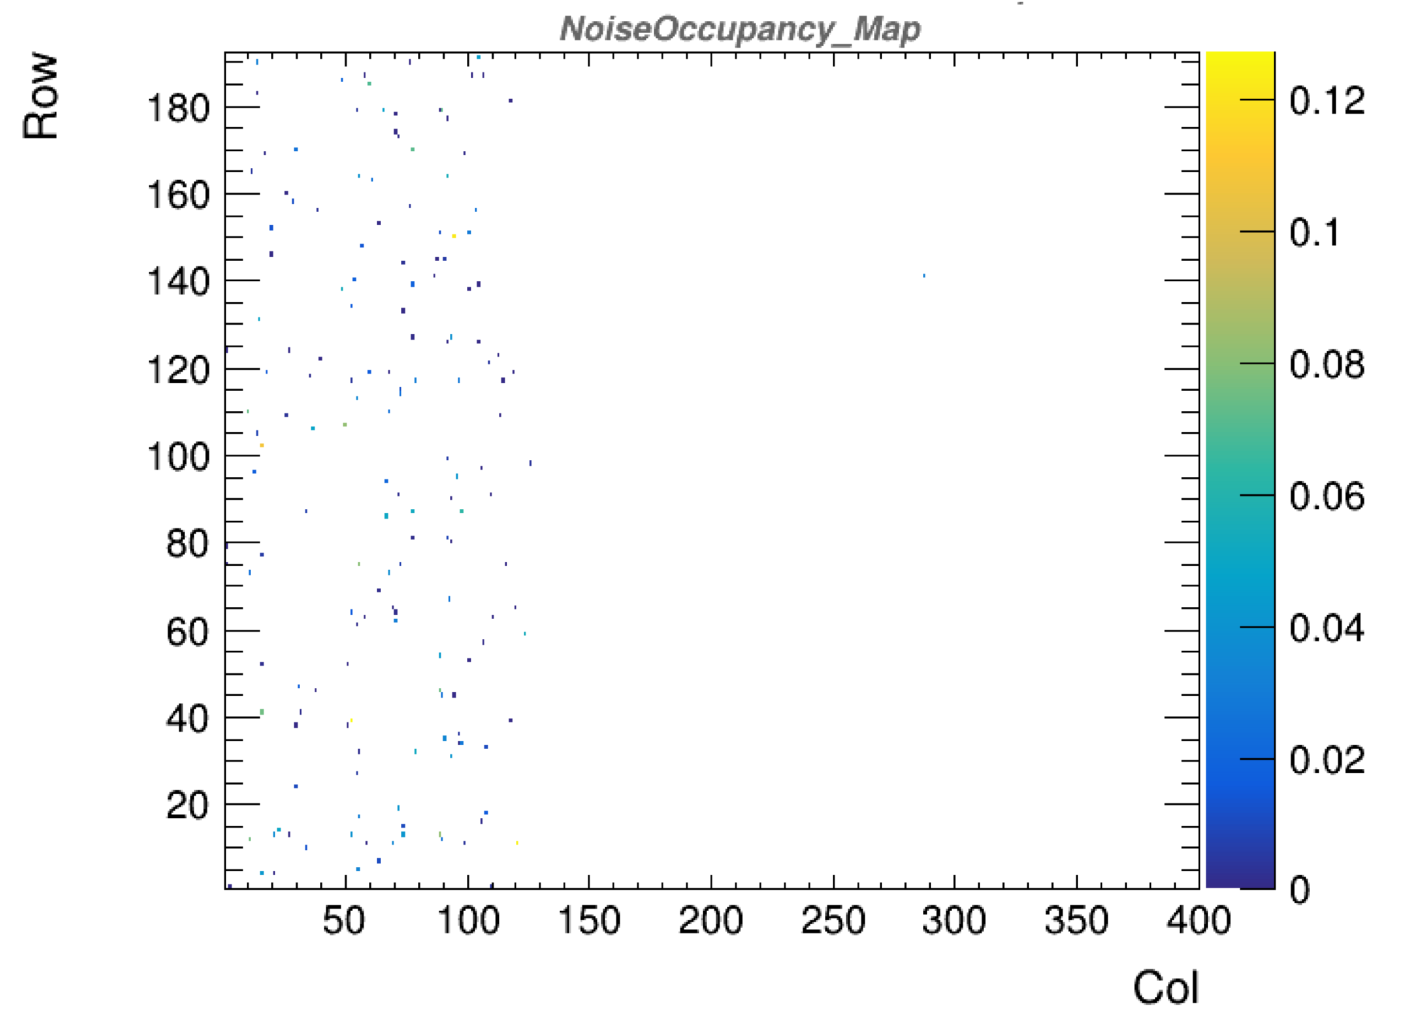
\includegraphics[width=8cm]{noise_occ}
\caption[ノイズ占有率測定における$NoiseOccupancy$分布の例。]{ノイズ占有率測定における$NoiseOccupancy$分布の例。図はRD53Aを用いたデジタル回路読み出しの結果であり、横軸、縦軸はそれぞれピクセルの列(400)、行(192)に対応する。z軸は各ピクセルにおける$NoiseOccupancy$の値を示している。正常なピクセルでは限りなく0に近い値になることが期待され、図ではほとんどのピクセルが0となっていが、列番号が0から120付近の領域で値を大きく持つピクセルが存在する。}
\label{noise_occ}
\end{figure}

出力される結果ファイルを以下に示す。
\begin{description}
  \item [OccupancyMap] 各ピクセルの$Occupancy$を記す.
  \item [NoiseOccupancyMap] 各ピクセルの$NoiseOccupancy$を記す.
  \item [NoiseMask] $NoiseOccupancy < 10^{-6}$のピクセルを1、それ以外を0とした値を記す.
\end{description}
  
\subsubsection{Threshold調整とピクセル解析}\label{sec:pixel_analysis}
今後この論文では、この試験を読み出し試験と呼ぶ。
以下の流れで読み出しを行う。
\begin{itemize}
  \item デジタル回路読み出し
  \item アナログ回路読み出し
  \item Threshold測定
  \item Thresholdグローバルレジスタ調整
  \item Thresholdピクセルレジスタ調整
  \item ToTグローバルレジスタ調整
  \item Thresholdグローバルレジスタ再調整、精密調整
  \item Threshold測定
  \item スタックピクセル測定
  \item クロストーク測定
\end{itemize}

測定後、試験結果の解析を行い、モジュール上の各ピクセルが正常かどうかを判断する。
設定されている評価基準を表\ref{pixel_analysis_criteria}に示す。不良ピクセルには評価基準に応じた評価名が付けられる。

\begin{table}[tbp]
\begin{center}
\caption[ピクセル解析の評価基準一覧]{ピクセル解析の評価基準一覧\cite{3-1}。読み出し試験において各ピクセルが正常に機能しているかを判断するためにピクセル解析を行う必要があり、それの判断基準が表のように定義されている。この基準一覧は不良評価であり、全ての基準に当てはまらないピクセルが健康と判断される。不良ピクセルの数や分布は、モジュールの品質を決定する1つの要素となり、ITkに搭載するモジュールや配置の決定に用いられる。}
\label{pixel_analysis_criteria}
  \scriptsize
  \begin{tabular}{|lll|} \hline
    評価名 & 読み出し項目 & 評価基準 \\ \hline
    Digital Dead      & Digital scan           & $Occupancy < 1$ \\ \hline
    Digital Bad       & Digital scan           & $Occupancy < 98 \: or \: Occupancy > 102$ \\\hline 
    Merged Bump       & Analog scan            & $Occupancy < 98 \: or \: Occupancy > 102$  \\ 
                      & Crosstalk scan         & High Crosstalk\\ \hline
    Analog Dead       & Analog scan            & $Occupancy < 1$ \\ \hline
    Analog Bad        & Analog scan            & $Occupancy < 98 \: or \: Occupancy > 102$ \\ \hline
    Tuning Failed     & Threshold scan         & Sカーブフィット失敗(YARRでは$\chi^2=0$となる) \\ \hline
    Tuning Bad        & Thresheld scan         & $|Q_{\rm th}-Q_{\rm th,mean}| > 5 \times Q_{\rm th,sigma}$ \\ 
                      & ToT scan               & ToT $ = 0 \: or \: 15 $\\ \hline
    High ENC          & Threshold scan         & $|\sigma_{\rm n}-\sigma_{\rm n,mean}| > 3 \times \sigma_{\rm n,sigma}$\\ \hline
    Noisy             & Noise scan             & $NoiseOccupancy > 10^{-6}$\\ \hline
    Disconnected Bump & Disconnected bump scan & 現段階では未決定 \\ 
                      & Source scan            & $Occupancy$がFEチップ全体平均の$1\%$ \\ \hline
    High Crosstalk    & Crosstalk scan         & $Occupancy>0 \: with \: 25{\rm ke}$ (sync FE)\\
                      &                        & $Occupancy>0 \: with \: 40{\rm ke}$ (lin and diff FE)\\ \hline 
  \end{tabular}
\end{center}
\end{table}

\subsubsection{簡易読み出し試験}
簡易読み出し試験では以下の項目を扱う。
\begin{itemize}
  \item レジスタの読み書き
  \item デジタル回路読み出し
  \item アナログ回路読み出し
  \item Threshold読み出し
  \item ToT読み出し
  \item バンプ接続確認読み出し
\end{itemize}

\subsubsection{バンプ接合確認試験}
放射線源を用いてバンプ接合の確認を行う。
以下の項目を扱う。
\begin{itemize}
  \item バンプ接合確認測定
  \item ノイズ占有率測定測定
  \item 外部トリガーを用いた測定
\end{itemize}

\subsection{各組み立て工程における品質試験}

各組み立て工程と品質試験項目を図\ref{stage_test_flow}に示す。
図より、1モジュールに対して行われる品質試験は30程度存在することが分かる。

\begin{figure}[bpt]\centering
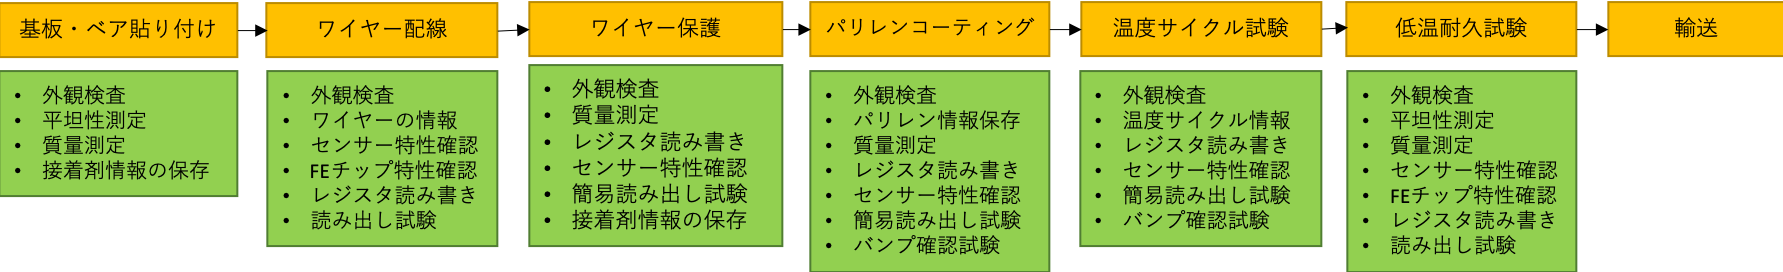
\includegraphics[width=15cm]{stage_test_flow}
\caption[組み立て工程と対応する品質試験一覧]{組み立て工程と対応する品質試験一覧。章\ref{sec:assembly}で述べた各組み立て工程において、複数の品質試験を行う必要がある。図は各組み立て工程と対応する品質試験一覧を示している。試験数は30程度存在する。}
\label{stage_test_flow}
\end{figure}

\section{検出器量産におけるデータ管理}
各組み立て機関で$O(100)〜O(1,000)$のモジュールを作り、上述したように1モジュールに対して30程度の品質試験を行う。
1,000モジュール作る機関であれば3,000の試験結果が得られる。この数の品質試験結果を正確に管理することが必要となる。
特に読み出し試験については、1試験につき更に細かい項目に細分化され、項目数、結果ファイル数も多様である。
これらの情報は最終的に共通のデータベースに保存する必要があり、各組み立て機関で適切に管理する必要がある。

本研究では各組み立て機関におけるモジュール情報及び品質試験のデータ管理を簡易化することを目的として、データベースシステムの構築を行った。
このシステムについて\ref{chap:dbsystem}章で記述する。

